%---------------------------------------------------------------------------------------------------
% Hauptteil
%---------------------------------------------------------------------------------------------------
%\newpage
%%\part{Hauptteil}

% Kapitel 1: Von der Integration zur Inklusion - eine Begriffserkl�rung 
\chapter{Sozial-emotionale Kompetenzen: Begriffserkl\"arung}
  \begin{flushleft}
    Da soziale Kompetenz und emotionale Kompetenz sehr stark miteinander verwoben sind, werden sie oft zusammen betrachtet. Doch im folgenden Verlauf m�chte ich des Verst�ndnisses wegen, diese beiden zwar sehr eng verbundenen, aber doch unterschiedlichen Kompetenzbereiche getrennt voneinander betrachten.
  \end{flushleft}
  \newpage
  \section{Emotionale Kompetenz}\label{sec:2_1}
    \begin{flushleft}
      Sich ein Bild von der Welt zu machen ist ein bedeutender Entwicklungsschritt in der fr�hen Kindheit. Hierzu geh�rte es zu lernen, mit den eigenen und den Gef�hlen anderer umzugehen. Daher spielt die F�rderung und Bildung von emotionaler Kompetenz eine wichtige Rolle in der Fr�hkindp�dagogik. Im Verlauf der emotionalen Entwicklung bilden sich bei Kindern F�higkeiten und Fertigkeiten aus, die zu emotionaler Kompetenz f�hren. \citep[vgl.][S.~13ff]{EmotionaleK2008} Vom S�uglingsalter bis hin zum Eintritt in die Schule erwerben Kinder die F�higkeit... sich ein Bild von sich selbst in dieser zu Welt machen, sich ein Bild von anderen in dieser Welt zu mache und das Weltgeschehen zu erleben, zu erkunden und gemeinsam mit anderen verantwortlich zu gestalten. \citep[zitat][S.~15]{HamburgBil2012} Dies tun sie in dem sie sich ihrer eigenen Gef�hle bewusst werden, ihren Gef�hlen durch Mimik oder Sprache Ausdruck verleihen, ihre Emotionen regulieren und die Gef�hle anderer Menschen erkennen und verstehen. Wie wichtig der angemessene Erwerb von emotionaler Kompetenz ist, vor allem f�r das Sozialverhalten, zeigen zahlreiche Studien. Aus ihnen geht hervor, dass eine hohe emotionale Kompetenz einhergeht mit einer positiven sozialen Kompetenz. \citep[vgl.][S.~13ff]{EmotionaleK2008} 
    \end{flushleft}

  \section{Soziale Kompetenz}
    \begin{flushleft}
      Die Grundlage f�r die sozialen Kompetenzen, sind die emotionale Kompetenzen. Um der Aufgabe zwischenmenschlicher Beziehungen gerecht zu werden, wird vorausgesetzt, dass mit den eigenen und den Gef�hlen von anderen Menschen umgegangen werden kann. Soziale Kompetenz bezeichnet ein breites Feld an pers�nlichen F�higkeiten. So verh�lt sich eine Person sozial kompetent, wenn sie in der Lage ist, ihr individuelles Interesse mit den Einstellungen, Werten und Normen einer Gruppe zu verkn�pfen. \citep[vgl.][S.~5]{SozioemoK2012} Daher ist es auch nicht verwunderlich, dass soziale Kompetenzen sehr von dem Rahmen abh�ngen sind, in dem sich die Person befindet. Was zum Beispiel in einem Moment oder einer Kultur als sozial kompetent gilt, kann an einem anderen Ort zu einer anderen Zeit genau das Gegenteil bedeuten. Wie bereits in Abschnitt \ref{sec:2_1} erw�hnt, setzt eine hohe soziale Kompetenz eine hohe emotionale Kompetenz vorraus. Doch was genau bedeutet das f�r ein Kind in unserer Gesellschaft? Eine bessere Akzeptanz und Einfluss bei Gleichaltrigen, die Kontaktaufnahme und -aufbau mit anderen f�llt leicht. Es kann ohne weiteres in neue Spielsituationen hineinfinden. Es kann sich in andere hineinf�hlen und versteht soziale Situationen. Hierf�r sind F�higkeiten wie \gls{Empathie} zu empfinden und Konflikte austragen zu k�nnen entscheidend. \citep[vgl.][S.~12ff]{SozialemoE2012}
    \end{flushleft}
    \subsection{Konflikte}\label{sec:2_2_1}
      \begin{flushleft}
        Unser Alltag ist von Konflikten bestimmt und gerade der Kita-Alltag bietet ausreichend Potential f�r Streiterein und freudige Auseinandersetzungen. Dies ist aber bei weitem nichts schlechtes, es ist eher der beste Beweis f�r ein aktives Sozialleben der Kinder. \citep[vgl.][S.~58]{Bildungsb2004} So geraten Kinder unteranderem im gemeinsamen Spiel h�ufig an ihre Grenzen, da sie hier ihre Interessen durchsetzen wollen - siehe auch Abschnitt \ref{sec:3_1} und Abschnitt \ref{sec:3_3_1}. Sei es jetzt nun das Spielzeug, das sie haben wollen oder das Durchsetzen eigener Bed�rfnisse und Interessen, all dies bietet ausreichend Konfliktpotential. Auch wenn Konflikte oft in Missverst�ndnissen und Entt�uschung m�nden, sind sie wichtig f�r die sozial-emotionale Entwicklung. Ja, man mag es fast nicht glauben, aber vom richtigen Streiten k�nnen Kinder viel lernen. \citep[vgl.][S.~10]{BedeutSpiel2011} Hier ist nat�rlich die Voraussetzung, dass Kinder streiten d�rfen und der Streit nicht als etwas per se schlechtes gesehen wird. Wenn Kindern der Raum f�rs Streiten bzw. austragen von Konflikten geboten wird und das p�dagogische Fachpersonal signalisiert \enquote{Wir sind da wenn ihr Unterst�tzung braucht}, k�nnen Kinder wichtige Kompetenzen entwickeln. Doch was lernen Kinder aus Konflikten? Nach Simone Pfeffer lernen Kinder unteranderem, ihre Bed�rfnisse zu �u�ern, sich mit anderen Kindern auf Spielregel zu einigen  bzw. sie gemeinsam auszuhandeln und L�sungen daf�r zu finden. Des Weiteren lernen sie, sich in Gruppen zu behaupten in dem sie eigene Interessen durchsetzen oder aber auch verschiedene Interessen wahrnehmen und diese verhandeln. Dadurch lernen sie Teil einer Gruppe zu sein, aber gleichzeitig sich von den Gef�hlen der anderen Kinder abzugrenzen. Au�erdem bieten Konflikte Kindern eine weitere Chance ihr eigenes Selbstkonzept zu entwickeln. \citep[vgl.][S.~42]{SozialemoE2012} All diese Strategien und L�sungsm�glichkeiten k�nnen f�r das gesamte sp�tere Leben eine tragf�hige Basis bilden.
      \end{flushleft}
  \newpage
  \section{Sozial-emotionale Kompetenzen ein lebenslanger Prozess}
    \begin{flushleft}
      Inwieweit sozial-emotionale Kompetenzen entwickelt sind, ist f�r alle Lebensbereiche von gro�er Wichtigkeit, sowohl f�r den Einzelnen, wie auch aus gesellschaftlicher Sicht. In welcher Qualit�t Kinder und Erwachsene Beziehungen zu andern Menschen erleben und gestalten d�rfen, steht in direkten Zusammenhang mit ihren sozial-emotionalen F�higkeiten. Dies betrifft alle Beziehungen, die Kinder und Erwachsene im Laufe ihres Lebens f�hren werden. Damit sind sowohl die Beziehungen gemeint, die im privaten Rahmen geschlossen werden, wie die Familie und Freunde, als auch die Beziehungen die im Kindergarten, der Schule oder sp�ter auch im Berufsleben geschlossen werden. \citep[vgl.][S.~14]{SozialemoE2012}
    \end{flushleft}

    \begin{flushleft}
      Die F�higkeit Gef�hle anderer erkennen und benennen zu k�nnen, hat auf lange Sicht eine positive Wirkung auf die sozial-emotionalen F�higkeiten von Kindern. Dies spiegelt sich auch in verschiedenen Untersuchungen wider, die aufzeigen inwieweit umfangreiches Emotionswissen und das Erkennen von Emotionen im mimischen wie auch sprachlichen Ausdruck, sich positiv auf die soziale Kompetenz auswirkt. Einhergehend damit ist die hohe Akzeptanz bei Gleichaltrigen, mehr soziale Kontakte zu Gleichaltrigen und gleichzeitig weniger aggressives Verhalten gegen�ber ihren Altersgenossen. \citep[vgl.][S.~23]{EmotionaleK2008} Eine entscheidende  Rolle hierbei spielt die Kommunikation. Diese, ob nun non-verbale oder verbale, ist das Medium f�r soziales Handeln. Soziale Kontakte und Beziehungen k�nnen hier durch sowohl gef�rdert, als auch zerst�rt werden, auch dann wenn, nichts verbal ge�u�ert wird. Denn man kann nicht nicht kommunizieren, jede Handlung ist auf ihre Art Kommunikation. \citep[vgl.][S.~6]{SozioemoK2012} Uneindeutigkeiten oder falsche Interpretationen von Kommunikationen, k�nnen zu Missverst�ndnissen und Konflikten f�hren. Zu Aggressionen und Konflikten kann es auch durch das Nicht-Wahrnehmen und Respektieren von Grenzen f�hren. Des Weiteren erden f�r die soziale-emotionalen F�higkeiten von Kinder positives Selbstbild vorrausgesetzt. Wenn ein Kind dies nicht hat, wird es viel mehr damit besch�ftigt sein, sein eigenes Selbstbild zu regulieren, als seiner Umwelt neugierig, offen und aufnahmebereit entgegenzutreten. \citep[vgl.][S.~14]{SozialemoE2012} Studien haben gezeigt, dass dies in direkten Zusammenhang mit schulischen Erfolgen steht. Kinder, die �ber keine guten sozial-emotionalen Kompetenzen verf�gen, haben weniger Leistungserfolge und sie erreichen meist nur eine unzureichende Schulreife. Zudem haben sie Schwierigkeiten, sich im Klassenverband einzuf�gen und geraten eher mit ihren Mitsch�lern in Konflikte.  \citep[vgl.][S.~27]{EmotionaleK2008}
    \end{flushleft}
    \begin{center}
      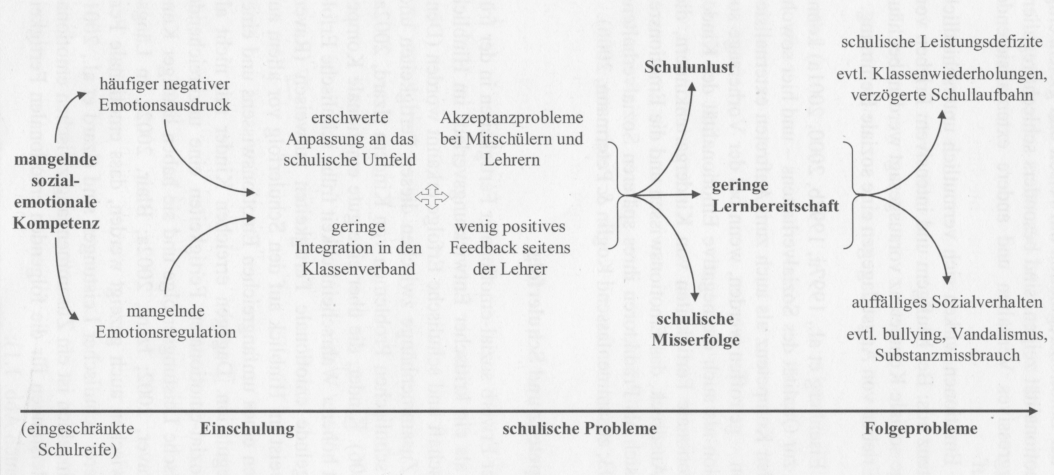
\includegraphics[width=1.0\textwidth]{grafik/shirin_grafik.pdf}
      \captionof{figure}[Zusammenhang mangelnder sozial-emotionalen Kompetenz und Schulproblemen]{Aus der folgende Grafik wird deutlich in welchen Zusammenhang mangelnder sozial-emotionalen Kompetenz und Schulproblemen stehen \citep[vgl.][S.~28]{EmotionaleK2008}}
      \label{fig:zusammenhang}
    \end{center}
    \begin{flushleft}
      Bildung hat in unserer heutigen Gesellschaft einen sehr hohen Stellenwert. Der schulische Erfolg jedes Einzelnen hat weitreichende Konsequenzen f�r sein Leben und f�r das bestehen der Gesamtgesellschaft. So steht Arbeitslosigkeit in direkter Korrelation mit Schulmisserfolg. Dies zeigt, dass der fr�hzeitige Erwerb von sozial-emotionalen Kompetenzen sehr wichtig ist, da sie eine Basis f�r die kindliche Entwicklung bilden und einen nachhaltigen Einfluss auf den Lebensverlauf haben. \citep[vgl.][S.~15]{SozialemoE2012}
    \end{flushleft}

\newpage

% Kapitel 2: Fehldeutungen und Chancen von Inklusion				
\chapter{Erwerb und F�rderung von sozial-emotionalen Kompetenzen durch Spiel und Bewegung}
  \begin{flushleft}
    K�rpererfahrungen sind Selbsterfahrungen. Spiel und Bewegung stellen f�r Kinder grundlegende Bet�tigungsformen, zugleich aber auch elementare Medien ihrer Erfahrungsgewinnung und ihrer Ausdrucksm�glichkeiten dar.
  \end{flushleft}
  \section{Was wird unter Spiel verstanden}\label{sec:3_1}
    \begin{flushleft}
      Solange es Menschen gibt wird und wurde, �berall auf der Welt und zu jeder Zeit, gespielt. Kinder entdecken durch das Spiel sich und ihre Umwelt. Sie erforschen, begreifen und erobern sich und die Welt, bei der Auseinandersetzung mit ihrer Umwelt. So ist das Spiel keine angeborene T�tigkeit, sondern eher das Produkt ihrer eigenen Neugier. \citep[vgl.][S.~4]{BedeutSpiel2011} In den Hamburger Bildungsempfehlungen wird daraufhingewissen, dass das Spielen die wohl bedeutsamste und wirkungsvollste Art des Lernens ist. Kindern sollte deswegen gen�gend Zeit und Raum zur Verf�gung gestellt werden, um zu spielen. Denn Spielen ist keine Spielerei, Kinder lernen hier wichtige F�higkeiten f�r ihr Leben. \citep[vgl.][S.~30]{HamburgBil2012} \enquote{\textit{Das Spiel ist Lernen mit allen Sinnen, mit starker emotionaler Beteiligung, mit geistigem und k�rperlichem Krafteinsatz.}} \citep[Zitat:][S.~30]{HamburgBil2012}
    \end{flushleft}
  \newpage
  \section{Bewegung -- Bet�tigungs- und Ausdrucksform von Kindern}
    \begin{flushleft}
      Ohne Bewegung k�nnte der Mensch nicht existieren. Schon im Mutterleib beginnt die Bewegungsentwicklung und sie endet erst mit dem letzten Atemzug. Bewegung ist ein Begriff, der sehr viele unterschiedliche T�tigkeiten mit einbezieht. Auf der einen Seite stehen die sportlichen T�tigkeiten, wie Fu�ball spielen, Radfahren und laufen, die von den meisten Menschen als Sport wahrgenommen werden. Auf der anderen Seite geh�ren, aber auch solche Dinge wie essen, malen, schreiben und musizieren zum Bereich Bewegung. Wenn man es genau nimmt sind sogar Gef�hle Bewegungen des menschlichen K�rpers. So sind bei Weitem nicht nur sportliche Aktivit�ten Bewegung. Nein, der K�rper bewegt sich sogar bei einem vermeintlichen Stillstand -- das Blut flie�t, das Herz schl�gt, die Lungen atmen und das Gehirn arbeitet.
    \end{flushleft}

    \begin{flushleft}
      Zudem spielt Bewegung in unterschiedlichen Lebensphasen eine mehr oder weniger gewichtige Rolle. So ist es f�r Kinder noch sehr wichtig sich viel zu bewegen und das kurze Stillsitzen kann sie vor eine innere Zerrei�probe stellen. Wohingegen �ltere Menschen sich gerne hinsetzten und ausruhen. Auch die Bedeutung von Bewegung ver�ndert sich, so h�ngt sie vom Lebensalter und den Lebensbedingungen ab. Durch ihre vielf�ltige Funktion, spielt sie gerade f�r die Entwicklung von Kindern eine gro�e Rolle. Im Folgenden werde ich nur darauf eingehen, welche Funktion Bewegung f�r die sozial-emotionalen Kompetenzen hat. Durch die Auseinandersetzung mit den eigenen k�rperlichen F�higkeiten lernen Kinder sich und ihren eigenen K�rper kennen. So gelingt es ihnen durch Bewegung, ihr \gls{Selbstbild} zu bilden und zu st�rken. Darauf aufbauend, k�nnen Kinder ihre sozialen F�higkeiten, durch gemeinsames Tun, das Spielen gegen- und miteinander und das verbalen Auseinandersetzen mit anderen (an- und absprechen, nachgeben und sich durchsetzen), aufbauen und erweitern- zu diesem Thema siehe auch Abschnitt \ref{sec:3_1}. \citep[vgl.][S.~16]{Handbuch2012}
    \end{flushleft}
  \newpage
  \section{Durch Spiel und Bewegung sozial-emotionale Kompetenzen erwerben}
    \begin{flushleft}
      Die Kindergartenzeit ist ein wichtiger Lebensabschnitt, hier eigenen sich Kinder unbewusst soziales Verhalten an. Dies geschieht durch den Aufbau neuer sozialer Beziehungen und Lernprozesse die in Gang gesetzt werden. Beeinflusst wird es durch die Erfahrungen, die sie im allt�glichen Umgang mit P�dagogen und Kindern machen. So bieten gerade Kinderg�rten eine gute Voraussetzung f�r den Erwerb sozial-emotionaler Kompetenzen. \citep[vgl.][S.~6f]{SozioemoK2012} Denn hier haben Kinder die M�glichkeit von Kindern zu lernen. Gerade altersgemischte Gruppen bieten sich daf�r an, sich gegenseitig zu helfen und zu unterst�tzen, sowie  die F�higkeiten der anderen einsch�tzen zu lernen.
    \end{flushleft}

    \begin{flushleft}
      Durch Spielen und Bewegen k�nnen Kinder Grundregeln des Sozialverhaltens erlernen und erproben. Kinder werden durch unterschiedlichste Spiel- und \gls{Bewegungsangebote} dazu angehalten, sich mit ihren Spielpartnern auseinanderzusetzen. So stehen sie vor der Herausforderung verschiedene Aufgaben zu bew�ltigen, wie etwa Konflikte zu f�hren und zu l�sen. Zu dem Thema Konflikte siehe auch Abschnitt \ref{sec:2_2_1}. Au�erdem lernen sie verschiedene Rollen zu �bernehmen und sich im Spiel mit Regel auseinanderzusetzen, indem die sie diese aushandeln und anerkennen. \citep[vgl.][S.~34f]{Handbuch2012} Diese entscheidenden Lernprozesse k�nnen bewusst, durch Spiel und Bewegung, initiiert und gestaltet werden. Im Spiel, sowohl im Freispiel als auch im angeleiteten Spiel, bekommen Kinder die M�glichkeit, neue Regel und Verhaltensweisen zu erproben und verinnerlichen. Es ist wichtig zu wissen, dass Kinder es nicht als \enquote{Lern- oder Trainingseinheit} wahrnehmen. \citep[vgl.][S.~6f]{SozioemoK2012} \enquote{\textit{Ein Kind lernt beim Spielen. Es spielt jedoch nie, um zu lernen, sondern weil es Freude an seiner T�tigkeit empfindet.}} \citep[Zitat:][S.~89]{Handbuch2012}
    \end{flushleft}

    \begin{flushleft}
      Beim Erwerb und Erweitern von sozialen Verhalten, ist f�r Kinder Nachahmung ihrer Mitmenschen ein wichtiges Werkzeug. \citep[vgl.][S.~38]{Handbuch2012} Das p�dagogische Fachpersonal spielt hierbei eine entscheidende Rolle. Daher ist wichtig, dass sich die P�dagogen �ber den zentralen Stellenwert, den sie beim Erlernen von sozialen Verhalten einnehmen, bewusst sind. In diesem Zusammenhang ist es bedeutsam, dass das p�dagogische Fachpersonal R�ume, Anl�sse und Gelegenheiten schaffen, in denen Kinder soziales Handeln und Verhalten erproben und anwenden k�nnen. Hier bietet sich der p�dagogische Alltag an, da die F�rderung des sozial Verhaltens hier unabh�ngig von R�umen oder Materialien stattfinden kann. \citep[vgl.][S.~7]{SozioemoK2012}
    \end{flushleft}


    \subsection{Die Bedeutung vom Spiel mit Gleichaltrigen f�r die sozial-emotionale Entwicklung bei Kindern}\label{sec:3_3_1}
      \begin{flushleft}
        Grundbed�rfnisse des Menschen sind es, soziale Kontakte und \gls{Freundschaften} zu f�hren und zu pflegen. In Beziehungen \gls{Gleichaltrigen} machen Kinder Erfahrungen von Vertrautheit, N�he, Austausch, Auseinandersetzungen, Streit und Vers�hnung. F�r eine angemessene Entwicklung von sozial-emotionalen Kompetenzen ben�tigen Kinder andere Kinder. In Peerbeziehungen, machen die Kinder, anders als mit Erwachsenen, die Erfahrung gleichgestellt zu sein. Hier haben sie die Aufgabe Regeln, Rollen und Machtverh�ltnisse miteinander auszuhandeln. Wenn ihnen diese herausfordene Aufgabe nicht gelingt, kann es nicht zum Spiel kommen. \citep[vgl.][S.~50ff]{SozialemoE2012} Gerade Freunde bieten vielf�ltige Gelegenheiten, Spiele zu entwickeln und Ideen auszutauschen. Des Weiteren besch�ftigen sich Kinder in \gls{Freundschaften} mit komplexeren und kooperativeren Spielen, doch sie geraten auch h�ufiger aneinander, als mit Kindern mit denen sie nicht befreundet sind. Andererseits wissen sie wiederum bei Freunden eher wie sie zu einer L�sung kommen k�nnen, um Streitereien aus dem Weg zu r�umen. \citep[vgl.][S.~721]{Entwicklungspsy2005} Diese Streitereien k�nnen auch gerne mal heftig und lautstark ausgetragen werden, aber in der Regel bem�hen sich Kinder bestimmte Verhaltensregeln und Grenzen einzuhalten. Kinder, die ihre Emotionen nicht unter Kontrolle haben und aggressiv reagieren, haben keinen guten Stand bei ihren Altersgenossen. \citep[vgl.][S.~53]{SozialemoE2012} Dies zeigen auch zahlreiche Studien. Entwicklungsforscher haben bei der Erhebung des \gls{soziometrischen Status} von Kindern, herausgefunden, dass ein Teil der Kinder, die eher von den Gleichaltrigen abgelehnt wurden, h�ufig aggressives Verhalten zeigen. Kinder die durch Gleichaltrige, auf Grund von aggressiven Verhalten, abgelehnt wurden, litten auch h�ufiger unter sp�tern Schul- und Verhaltensproblemen. \citep[vgl.][S.~723,743]{Entwicklungspsy2005}
      \end{flushleft}
  \newpage
  \section{Durch Spiel und Bewegung sozial-emotionale Entwicklung f�rdern}
    \begin{flushleft}
      Am Anfang steht jedoch die Frage: Ist es �berhaupt m�glich sozial-emotionale Kompetenzen zu f�rdern oder ist es sinnlos dies zu versuchen, da Soziale Bildung sowieso ein Selbstbildungsprozess des Kindes ist? Die Annahme, dass soziale Bildung eine Selbstbildung ist, ist nicht von der Hand zu weisen, doch sollte nicht vergessen werden, dass dies unteranderem ebenfalls durch Anregungen von erwachsenen Bezugspersonen erlangt wird. Im Kindergarten bieten sich zwar h�ufig von selbst Gelegenheiten zum sozialen Lernen an. \citep[vgl.][S.~11]{SozioemoK2012} Doch was tats�chlich beim \gls{Freispiel} gelernt wird und was aus p�dagogischer Sicht gelernt werden sollte, unterscheidet sich derweilen. Beobachtungen von Freispielsitutionen zeigen, dass Kinder nicht nur positive Erfahrungen dabei machen. So werden Kinder ausgeschlossen, Machtpositionen werden ausgespielt und nicht alle W�nsche und Interessen werden ber�cksichtigt. Daher kann das fr�hp�dagogische Fachpersonal durch die Auswahl der Spiele, als auch durch die damit verbundenen organisatorischen Ma�nahmen dazu beitragen, die sozialen Beziehungen in der Gruppe zu f�rdern. \citep[vgl.][S.~40]{Handbuch2012} Gerade p�dagogisch angeleitete \gls{Bewegungsangebote} und \gls{Bewegungsspiele} bieten vielf�ltige Lernanregungen. Zum einen um die motorischen F�higkeiten der Kinder herauszufordern, zum anderen um ihre sozialen F�higkeiten zu f�rdern und zu unterst�tzen. Bei konkreten Spielideen seitens des p�dagogischen Fachpersonales kann geguckt werden inwieweit sie sozial-emotionale Kompetenzen f�rdern.
    \end{flushleft}
    
    \begin{flushleft}
      Eine Spielanalyse kann wie folgt aussehen:
      \begin{itemize}
        \item Inwieweit werden Kinder dazu ermutigt in diesem Spiel empathisch zu sein?
        \item Inwieweit werden verschiedene Rollen in diesem Spiel eingenommen und ausgehandelt?
        \item Wie sieht in diesem Spiel die Kontaktaufnahme unter den Kindern aus?
        \item Inwiefern ist es f�r dieses Spiel von N�ten, sich gegenseitig zu helfen und mit anderen zu kooperieren?
        \item Welche Regeln gibt es und m�ssen diese gegebenfalls mit den Kindern abgesprochen bzw. neu definiert werden?
      \end{itemize}
    \end{flushleft}
    \newpage
    \begin{flushleft}
      Die Spielanalyse  gibt nun Aufschluss dar�ber, wenn sowie welche Spielelemente ver�ndert werden, sodass die sozial-emotionale Kompetenzen gef�rdert werden k�nnen. Es sollte im Auge behalten werden,Konkurrenzverhalten und vergleichen von Leistungen zu vermeiden, dagegen sollte Kooperation eher gef�rdert werden. Zudem sollte �berlegt werden, wie sozial-emotionale Kompetenz im Kita-Alltag gef�rdert werden kann, sodass die ganze Kita ein Lernraum wird, in dem man sich in gesch�tzter Umgebung sozial bilden kann. Neben Ritualen im Alltag, kann auch eine Wutecke, die daf�r da ist einfach mal seine Wut oder auch schlechte Laune rauszulassen, in die Kita Einzug finden. Nat�rlich k�nnte es auch ein Pendant zur Wutecke geben, hier h�tten die Kinder und Erwachsenen z.B. die M�glichkeit Nettigkeiten zusagen. Wichtig ist es nicht aus den Augen zu verlieren, dass man Kindern soziale Kompetenzen nicht beibringen kann, aber f�r sie Gelegenheiten schaffen kann in denen sie sich ausprobieren k�nnen. \citep[vgl.][S.~12]{SozioemoK2012} \enquote{Soziale Kompetenz entwickeln hei�t, gemeinsam mit anderen zu wachsen.} \citep[Zitat:][S.~13]{SozioemoK2012} Daher ist es wichtig, dass die p�dagogischen Fachkr�fte einen selbstreflektierten Blick auf ihr eigenes Handel haben. Besonders im Zusammenhang mit der L�sung von sozialen Konflikten, da Kinder auch unbewusst Dinge, Handlungen und Verhaltensweisen aus ihrer sozialen Umgebung �bernehmen. \citep[vgl.][S.~38]{Handbuch2012}
    \end{flushleft}
    \newpage
    \subsection{Projekt: F�rderung sozial-emotionaler Kompetenzen in Bewegung}
      \begin{flushleft}
        SEKIB (Bewegungsorientierte F�rderung sozial-emotionaler Kompetenzen in der fr�hen Kindheit)
      \end{flushleft}
      \begin{flushleft}
        Der Frage, wie man durch Spiel und Bewegung sozial-emotionale Kompetenzen f�rdern kann, geht zurzeit das Projekt SEKIB nach. Das Projekt l�uft �ber einen Zeitraum von ca. 4 Jahren, begonnen hat es am 01.10.2010 und endet am 30.06.2014. Geleitet wird es von Prof. Dr. Renate Zimmer. An dem Projekt nehmen 15 Kindertageseinrichtungen im Raum Dortmund teil. Hierf�r werden durch Spiel und Bewegung Anl�sse geschaffen, die zu Interaktion und Kommunikation f�hren sollen. In diesem Zusammenhang soll der Zugang �ber K�rper und Bewegung geschaffen werden, sodass der Umgang mit dem eigenen K�rper dazu dient, seine nonverbal und verbal Ausdrucksf�higkeit zu verbessern. Des Weiteren soll die Selbst- und Fremdwahrnehmung, Impulskontrolle, Empathie und Rollen�bernahme sowie der Umgang mit Konflikten ge�bt und verbessert werden. Zu diesem Zweck wurden von �ber 100 Kindern die quantitative und qualitative Daten zu ihren Sozialverhalten erhoben. Zum einem wurde das Sozialverhalten durch Erzieherinnen und ihre Eltern eingesch�tzt, zum anderen mussten sich die Kinder selbst einsch�tzen. Erhoben wurde bzw. wird dies, einmal am Anfang und am Ende des Projektes. Zu Beginn wurde durch Experteninterviews mit den p�dagogischen Fachkr�ften, die Alltagsbelastungen durch das Verhalten der Kinder ermittelt. Die Projektinhalte wurden auf Grund dieser Ergebnisse so konzipiert, dass sie den Erwartungen der Teilnehmerinnen gerecht werden und auf die Probleme, die im Alltag geschehen, eingehen. \citep[vgl.]{Sekib2013}
      \end{flushleft}           
\newpage

% Kapitel 3: Fazit				
%---------------------------------------------------------------------------------------------------
% Zusammenfassung
%---------------------------------------------------------------------------------------------------
% \newpage
%%\part{Schluss}
\chapter{Res�mee}
  \section{Reflexion: Die Wichtigkeit von Studieninhalten f�r die Arbeit als Kita-Leitungskraft}
    \begin{flushleft}
      Die Verwendung eines Interviews und das drauf folgende Shadowing stellten sich als gute Methoden heraus, um das T�tigkeitsprofil einer Kita-Leitungskraft erforschen zu k�nnen. Besonders wichtig war mir zu erfahren, inwieweit die Studieninhalte des Bachelor Studienganges Bildung und Erziehung in der Kindheit auf die vielf�ltige und anspruchsvolle Arbeit einer Kita-Leitungskraft vorbereitet.
    \end{flushleft}

    \begin{flushleft}
      So konnte ich durch das Interview in Erfahrung bringen, dass sein eigenes Studium- Diplom Psychologie- inhaltlich f�r Herrn Strau� und seine Arbeit nicht so hilfreich war, wie er es sich erhofft hatte. Doch die praktischen Anwendungsgebiete wiederum haben ihn sehr geholfen, um vielen allt�glichen Gegebenheiten ad�quat begegnen zu k�nnen. Gerade das Selbststudium haben ihm Selbstst�ndigkeit, Analysef�higkeiten, Organisationsf�higkeiten und probleml�sungsorientiertes Handeln gelehrt. Auch ich bin der Meinung, dass das Selbststudium uns in vielerlei Hinsicht F�higkeiten und Fertigkeiten vermittelt, die f�r den Beruf der Leitungskraft sehr hilfreich sind. Wohingegen ich beim inhaltlichen Teil des Studiums nicht mit Herrn Strau� konform gehe. Den Ergebnissen der angewandten Methoden konnte ich ableiten, dass der ganze Managementsektor w�hrend des Studiums von Herrn Strau� eher stiefm�tterlich behandelt wurde und er sich sein Wissen durch Erfahrungen aneignen musst. Da dieser Teil der Arbeit aber in den letzten Jahren immer mehr an Bedeutung gewonnen hat, sieht er sich gezwungen eine Weiterbildung im Bereich Management zu machen. Diesem wurde im Studiengang Bildung und Erziehung in der Kindheit vorgebeugt, indem Studierende dieses Studienganges durch das Hauptfach Management mit diesem Bereich schon in Ber�hrung kommen. Auch Seminare wie Selbst- oder Beratungskompetenz vermitteln theoretisches Wissen, das f�r den praktischen Alltag hilfreich sein kann.
    \end{flushleft}

    \begin{flushleft}
      Ich m�chte jetzt aber auch nicht ohne weiteres behaupten, dass alle Studieninhalte Relevanz f�r den Leitungsberuf haben. Des Weiteren bin ich der Meinung, dass viele Inhalte im Studium bzw. in Vorlesungen und Seminaren nur angerissen werden und ich bei einem weiterf�hrenden Interesse an einem bestimmten Thema, auf das Selbststudium zur�ck greifen muss. 
    \end{flushleft}

    \begin{flushleft}
      Schlussendlich w�rde ich behaupten, dass das Studium uns vielerlei Mittel und Informationen mitgibt die wir selbst zu b�ndeln und eigenverantwortlich weiterzuf�hren haben. Dies sollte als gute Schule f�r die sp�tere Berufswelt gesehen werden. Denn auch hier m�ssen wir lernen, unser theoretisches Wissen im Praxisalltag richtig  anzuwenden.
    \end{flushleft}

  \section{Fazit}
    \begin{flushleft}
      Die Zielsetzung dieser Arbeit war es, das T�tigkeitsprofil einer Kita-Leitungskraft zu beleuchten. Dies wurde an Hand von Herrn Strau�, der die Leitungsposition in der Kindertagesst�tte �bernimmt, gemacht. Zu diesem Zweck wurde erst gekl�rt, wie das Arbeits- und der Aufgabenbereich einer Kita-Leitung aussieht. Im weiteren Verlauf wurde dann darauf eingegangen, welchen gesetzlichen Rahmen, auf Bundes- wie auch auf Landesebene, zu beachten sind, um eine Kita leiten zu k�nnen. Dem folgte die Darlegung der Ergebnisse, die in Folge des Interviews und des Shadowings erlangt wurden. Zudem wurde er�rtert wie die zentralen Kompetenzbereiche dieses T�tigkeitfelds aussehen. Anhand der sich aus dem Interview und Shadowing erschlie�enden Erkenntnisse, wurde noch beleuchtet, welche organisationale Managementdimensionen als Kita-Leitung zu erf�llen sind. Abschlie�end wurde reflektiert, inwieweit das Interview und Shadowing Erkenntnisse erbracht haben, welche Relevanz das Studium f�r die Leitungst�tigkeit hat. 
    \end{flushleft}

    \begin{flushleft}
      Durch die Hausarbeit konnte gezeigt werden, wie vielf�ltig und anspruchsvoll die T�tigkeiten einer Leitungskraft sind. Zudem konnte man sehen, dass die p�dagogische Arbeit mit Kindern kaum bis gar nicht mehr zum T�tigkeitsfeld geh�rt. Daher ist es auch nicht verwunderlich, dass eine Kita-Leitungskraft �ber umfangreiche Kompetenzen verf�gen muss. Diese braucht sie haupts�chlich, um den Kita-Alltag mit all seinen Facetten zu begegnen, organisieren und managen k�nnen.
    \end{flushleft}

    \begin{flushleft}
      Nun zu meinem pers�nlichen Fazit. Ich hatte mir von dieser Facharbeit erhofft, zwei Sachen zu erfahren. Zum einen war es mir wichtig zu erfahren, welchen Stellenwert das Studium f�r die Arbeit einer Leitungskraft hat. Zum anderen wollte ich wissen, wie der Alltag und die Aufgaben einer Leitungskraft aussehen, da ich selbst bis jetzt nur Erfahrungen in der p�dagogischen Arbeit am Kind gemacht habe. 
    \end{flushleft}

    \begin{flushleft}
      Durch die angewandten Methoden und Instrumente konnte ich beide Ziele zu meiner vollsten Zufriedenheit erf�llen. Ich hatte im Rahmen dieser Arbeit die Gelegenheit, viele Erkenntnisse �ber den Alltag und die Aufgaben eine Kita-Leitungskraft  zu erlangen. Des Weiteren konnte ich durch die Analyse und Reflexion der Ergebnisse sehr gut f�r mich herausfiltern, welchen Stellenwert dieses Studium und ein Studium an sich f�r die Arbeit als Leitung einer Kindertagesst�tte hat. Diese neu gewonnen Erkenntnisse sind von gro�er Bedeutung f�r meine sp�tere Berufswahl. 
    \end{flushleft}

  \section{Ausblick}
    \begin{flushleft}
      Durch die im Rahmen dieser Hausarbeit durchgef�hrte Untersuchungen, konnte ich mir ein erstes Bild von dem T�tigkeitsfeld einer Kita-Leitungskraft machen. Da dieses Bild aber nur �ber einen sehr kurzen Zeitraum gebildet wurde und ich noch gerne mehr Praxisbezogenes �ber diesen Beruf erfahren w�rde, steht f�r mich fest, dass ich gerne im folgenden Semester ein Praktikum in diesen Bereich machen m�chte.  
    \end{flushleft}
           
\newpage

% Kapitel 4: Kinder der Regenbogengruppe				
% \input{kapitel/hauptteil/kinder_regengruppe}           
% \newpage

% Kapitel 5: Familie				
% \input{kapitel/hauptteil/familie}           
% \newpage

% Kapitel 6: P�dagogische Arbeit				
% \input{kapitel/hauptteil/paedagogische_arbeit}           
% \newpage

% Kapitel 7: Umfeld der Praxiseinrichtung				
% \input{kapitel/hauptteil/umfeld}           
% \newpage



% \chapter{Hauptteil}
%   \begin{flushleft}
%     In diesem Kapitel wird noch einmal das Problem zusammengefasst und die in der vorliegenden Arbeit entworfene L�sung vorgestellt und bewertet. Zudem soll ein Ausblick auf m�gliche Weiterentwicklungen der hier aufgef�hrten L�sung vorgestellt werden.\citep{Cohn2010}
%   \end{flushleft}